\documentclass[journal]{vgtc}                % final (journal style)
%\documentclass[review,journal]{vgtc}         % review (journal style)
%\documentclass[widereview]{vgtc}             % wide-spaced review
%\documentclass[preprint,journal]{vgtc}       % preprint (journal style)

%% Uncomment one of the lines above depending on where your paper is
%% in the conference process. ``review'' and ``widereview'' are for review
%% submission, ``preprint'' is for pre-publication, and the final version
%% doesn't use a specific qualifier.

%% Please use one of the ``review'' options in combination with the
%% assigned online id (see below) ONLY if your paper uses a double blind
%% review process. Some conferences, like IEEE Vis and InfoVis, have NOT
%% in the past.

%% Please note that the use of figures other than the optional teaser is not permitted on the first page
%% of the journal version.  Figures should begin on the second page and be
%% in CMYK or Grey scale format, otherwise, colour shifting may occur
%% during the printing process.  Papers submitted with figures other than the optional teaser on the
%% first page will be refused.

%% These few lines make a distinction between latex and pdflatex calls and they
%% bring in essential packages for graphics and font handling.
%% Note that due to the \DeclareGraphicsExtensions{} call it is no longer necessary
%% to provide the the path and extension of a graphics file:
%% 
\includegraphics{diamondrule} is completely sufficient.
%%
\ifpdf%                                % if we use pdflatex
  \pdfoutput=1\relax                   % create PDFs from pdfLaTeX
  \pdfcompresslevel=9                  % PDF Compression
  \pdfoptionpdfminorversion=7          % create PDF 1.7
  \ExecuteOptions{pdftex}
  \usepackage{graphicx}                % allow us to embed graphics files
  \DeclareGraphicsExtensions{.pdf,.png,.jpg,.jpeg} % for pdflatex we expect .pdf, .png, or .jpg files
\else%                                 % else we use pure latex
  \ExecuteOptions{dvips}
  \usepackage{graphicx}                % allow us to embed graphics files
  \DeclareGraphicsExtensions{.eps}     % for pure latex we expect eps files
\fi%

%% it is recomended to use ``\autoref{sec:bla}'' instead of ``Fig.~\ref{sec:bla}''
\graphicspath{{figures/}{pictures/}{images/}{img/}{./}} % where to search for the images

\usepackage{microtype}                 % use micro-typography (slightly more compact, better to read)
\PassOptionsToPackage{warn}{textcomp}  % to address font issues with \textrightarrow
\usepackage{textcomp}                  % use better special symbols
\usepackage{mathptmx}                  % use matching math font
\usepackage{times}                     % we use Times as the main font
\renewcommand*\ttdefault{txtt}         % a nicer typewriter font
\usepackage{cite}

% additional package
\usepackage{hyperref}
\usepackage{subcaption}
\usepackage{listings}

\lstset{basicstyle=\footnotesize\ttfamily,breaklines=true}

%% We encourage the use of mathptmx for consistent usage of times font
%% throughout the proceedings. However, if you encounter conflicts
%% with other math-related packages, you may want to disable it.

%% In preprint mode you may define your own headline.
%\preprinttext{To appear in IEEE Transactions on Visualization and Computer Graphics.}

%% If you are submitting a paper to a conference for review with a double
%% blind reviewing process, please replace the value ``0'' below with your
%% OnlineID. Otherwise, you may safely leave it at ``0''.
\onlineid{0}

%% declare the category of your paper, only shown in review mode
\vgtccategory{Research}

%% Paper title.
\title{Comparison of Energy Consumption in Wi-Fi and Bluetooth Communication: A Case Study on Context Aware Building}

%% This is how authors are specified in the journal style

%% indicate IEEE Member or Student Member in form indicated below
\author{Guntur Dharma Putra}
\authorfooter{
%% insert punctuation at end of each item
\item
 Guntur Dharma Putra is an MSc Student in Computing Science at the Universtiy of Groningen. E-mail: g.d.putra@student.rug.nl.
}

%other entries to be set up for journal
\shortauthortitle{Putra: Comparison of Energy consumption of Wi-Fi and Bluetooth Communication in Context aware Building}
%\shortauthortitle{Firstauthor \MakeLowercase{\textit{et al.}}: Paper Title}

%% Abstract section.
\abstract{
Context awareness has been an interesting topic recently. Its ability to infer whether a person exists on a particular room or building is really important for smart building. The result shows that Bluetooth is 29.97\% more energy efficient than WiFi.


} % end of abstract

%% Keywords that describe your work. Will show as 'Index Terms' in journal
%% please capitalize first letter and insert punctuation after last keyword
\keywords{Context-aware, smart building, wi-fi, bluetooth low energy}

%% ACM Computing Classification System (CCS). 
%% See <http://www.acm.org/class/1998/> for details.
%% The ``\CCScat'' command takes four arguments.

% \CCScatlist{ % not used in journal version
%  \CCScat{K.6.1}{Management of Computing and Information Systems}%
% {Project and People Management}{Life Cycle};
%  \CCScat{K.7.m}{The Computing Profession}{Miscellaneous}{Ethics}
% }

%% Uncomment below to include a teaser figure.
  %  \teaser{
  %  \centering
  %  \includegraphics[width=16cm]{CypressView}
  %  \caption{In the Clouds: Vancouver from Cypress Mountain.}
  % }

%% Uncomment below to disable the manuscript note
\renewcommand{\manuscriptnotetxt}{}

%% Copyright space is enabled by default as required by guidelines.
%% It is disabled by the 'review' option or via the following command:
% \nocopyrightspace

% \vgtcinsertpkg

%%%%%%%%%%%%%%%%%%%%%%%%%%%%%%%%%%%%%%%%%%%%%%%%%%%%%%%%%%%%%%%%
%%%%%%%%%%%%%%%%%%%%%% START OF THE PAPER %%%%%%%%%%%%%%%%%%%%%%
%%%%%%%%%%%%%%%%%%%%%%%%%%%%%%%%%%%%%%%%%%%%%%%%%%%%%%%%%%%%%%%%%

\begin{document}

%% The ``\maketitle'' command must be the first command after the
%% ``\begin{document}'' command. It prepares and prints the title block.

%% the only exception to this rule is the \firstsection command
\firstsection{Introduction}

\maketitle
Smart building has been an interesting topic of research recently. One portion of research in smart home is occupancy detection, which aims to detect whether a person is present in a particular location. Its importance to detect user presence is crucial in the building energy management, since the building can manage energy allocation efficiently regarding how many persons are present.

Several methods have been proposed to overcome the occupancy detection. One of them makes use of Bluetooth Low Energy (BLE) beacon, as the beacon is useful because it always transmitting a unique data packet that indicates certain location information. Assuming that the users always bring mobile phone with them, an application can be installed on the mobile phone to scan a particular beacon, so that the application knows where currently the user is, then the application sends the data to the central server. The data can be analyzed later on to detect user presence.

Normally, the application sends the data to the server through HTTP communication done via Wi-Fi connectivity, as the BLE is already used to sense the beacon. No BLE utilization for data transmission to the server has been found. In fact, BLE is obviously more energy efficient compared to WiFi, as BLE is designed to be implemented in devices coupled with limited source of energy, e.g., battery.

% how this study is positioned.
This study tries to investigate BLE utilization for transmitting the occupancy data to the server. This study measures and compares the energy consumption of the mobile phone when performing data transmission via WiFif and BLE. A tailored application is developed and several possible scenario is also taken into consideration, such as number of detected sensor and user location relative to the server or access point. The result of this study may be useful for the future decision whether BLE will be implemented instead of WiFi to transmit occupancy data to the server.

%% \section{Introduction} %for journal use above \firstsection{..} instead
The rest of this report is structured as follows. Section~\ref{sec:related_work} presents other related work to this study. Methodology is described in section~\ref{sec:methodology}, while the results and discussion is discussed in section~\ref{sec:results_and_discussion}. Lastly, a conclusion is drawn in section~\ref{sec:conclusion}

\section{Related Work} % (fold)
\label{sec:related_work}
cite all the related work properly that you base your own work on

discuss why it is relevant and what is similar or different to your own work
use images (from other papers) to illustrate the related work, credit the authors with a reference in the image caption

give details for each publication (authors, title, year, page numbers, publisher, publisher address (town); for articles volume and number and month; for things other than books, articles, or papers also the type of publication)

% section related_work (end)

\section{Methodology} % (fold)
\label{sec:methodology}
As a term project, this study was performed in three consecutive months. The main part of this study, the energy measurement, was carried out in iPhone 6, which runs iOS operating system. Additionally, Asus vivo mini PC, which runs Xubuntu as its operating system, was also utilized as a thin client that hosts the server application.

\subsection{System Architecture} % (fold)
\label{sub:system_architecture}
This study is based on a study from Azkario, which attempts to extract occupancy data in smart building. This system consist of BLE beacons, which are placed accordingly in each room, a user's mobile phone, and a sensing infrastructure, which consists of WiFi infrastructure and sensing server. Currently, the user's mobile phone uses HTTP over WiFi to send occupancy data to the server, while Bluetooth is only used in mobile phone to or from BLE beacons. The Bluetooth communication in this study is intended to replace the mobile phone to server that is currently implemented using HTTP over WiFi. Briefly, the system architecture is depicted in Figure~\ref{fig:system-architecture}. 

% To-Do add the sensing infrastructure on the right hand side
% add color as well, to the thin client
% add a dashed box to indicate where does this study reside
\begin{figure}
  \centering
    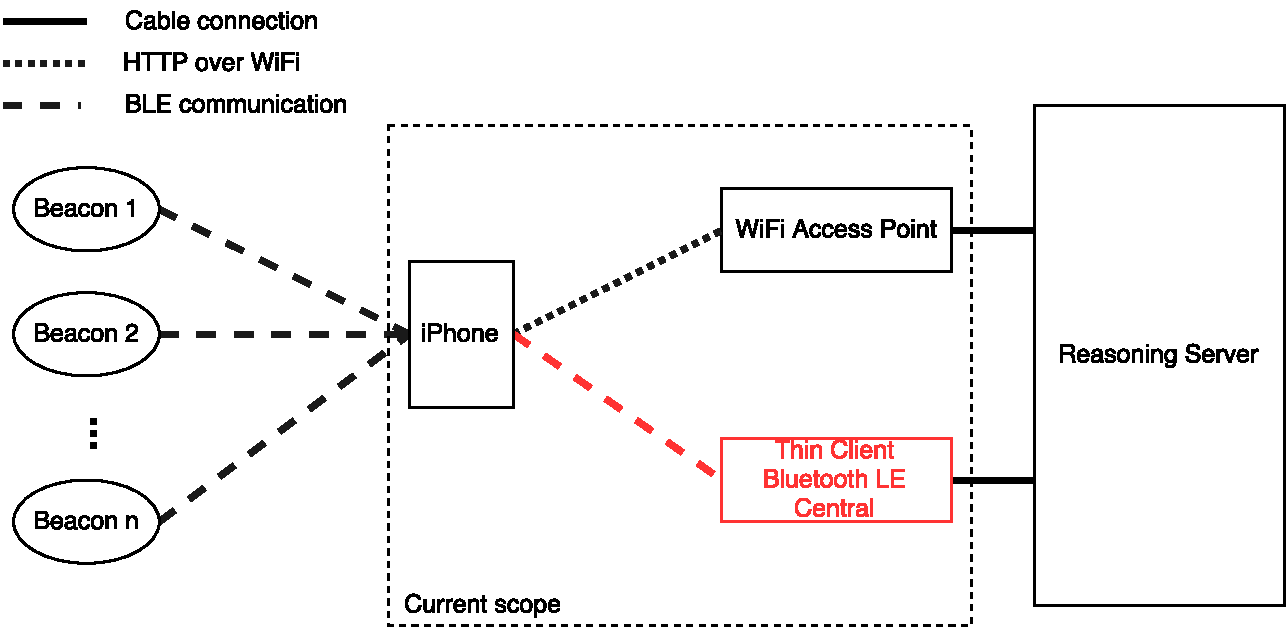
\includegraphics[width=0.45\textwidth]{system-architecture}
  \caption{System architecture overview.}
  \label{fig:system-architecture}
\end{figure}

As seen in Figure~\ref{fig:system-architecture}, the thin client (colored in red), which acts as BLE central, is added to the Azkario's architecture. Later, energy consumption between BLE and WiFi are measured and compared. Although the result may be obvious that BLE is more energy efficient than HTTP over WiFi communication, this study aims to figure out how efficient is BLE communication compared to HTTP over WiFi in this context.

This study only focuses on mobile phone (iPhone) to WiFi Access Point (for HTTP over WiFi) or Thin Client (for BLE communication) for energy consumption measurement, which is surrounded in dashed box. The sensing part of the whole architecture, which is from beacons to iPhone, is neglected. As a consequences, dummy data that imitates the real data from beacons is used, which is sent from the mobile phone in every second.
% subsection system_architecture (end)

\subsection{Measuring the Energy Consumption} % (fold)
\label{sub:tracing_}
Energy consumption measurement or tracing is the core of this study. It is done by using untethered energy logging in iOS, in which the energy consumption data is logged internally in the device itself before imported to the computer by using cable connection. This method is selected because it has the flexibility over the other methods. Wireless logging, which does not involve internal logging in the device, is not used as it requires Bonjour enabled router that was unavailable.

% how to measure
Apple's Instrument application in Mac OS X was used to import the logged energy measurement in iPhone, as done in~\cite{Conte2014}. It does not show the measurement result in standard energy measurement format, e.g., mAh, but it shows that in its own format, which is scaled from 0 to 20. Each increment in the scale costs an hour of battery life~\cite{Lucchesi2014}. Thus, phone running at level 1/20 will have 20 hours of battery life, while phone running at level 20/20 will have only 1 hour of battery life.

Furthermore, export feature is limited in Apple's Instrument, i.e., it does not support energy consumption log exporting to other commonly used format, e.g., csv or xls file. However, manual copying and pasting on each row is still supported. An Apple script was used to automate the copying and pasting the energy log to Excel for further processing. However, it was also not stable. It encountered several errors during its runtime, which were caused by OS instability, and restarting the process was only way to overcome that.
% probably put a pseudo code, if it has some logic

\subsubsection{Measurement Parameters} % (fold)
\label{ssub:measurement_parameters}
% what are the parameters? and why?
Some parameters were selected for measuring energy consumption, which are number of beacon and distance of communication. Three number of beacons are selected, which are 5, 10, and 20, because five beacons are the most common number of beacon sensed in real case, while 10 and 20 are the double size of it. Distance of communication is divided into two category, Line of Sight (LoS) and non-LoS. Line of Sight is a communication in which both communication endpoints can see each other without obstacle, while non-LoS means otherwise. Each of category has three distance. The set up of the measurement experiment is shown in Figure~\ref{fig:experiment-map}.

\begin{figure}
  \centering
    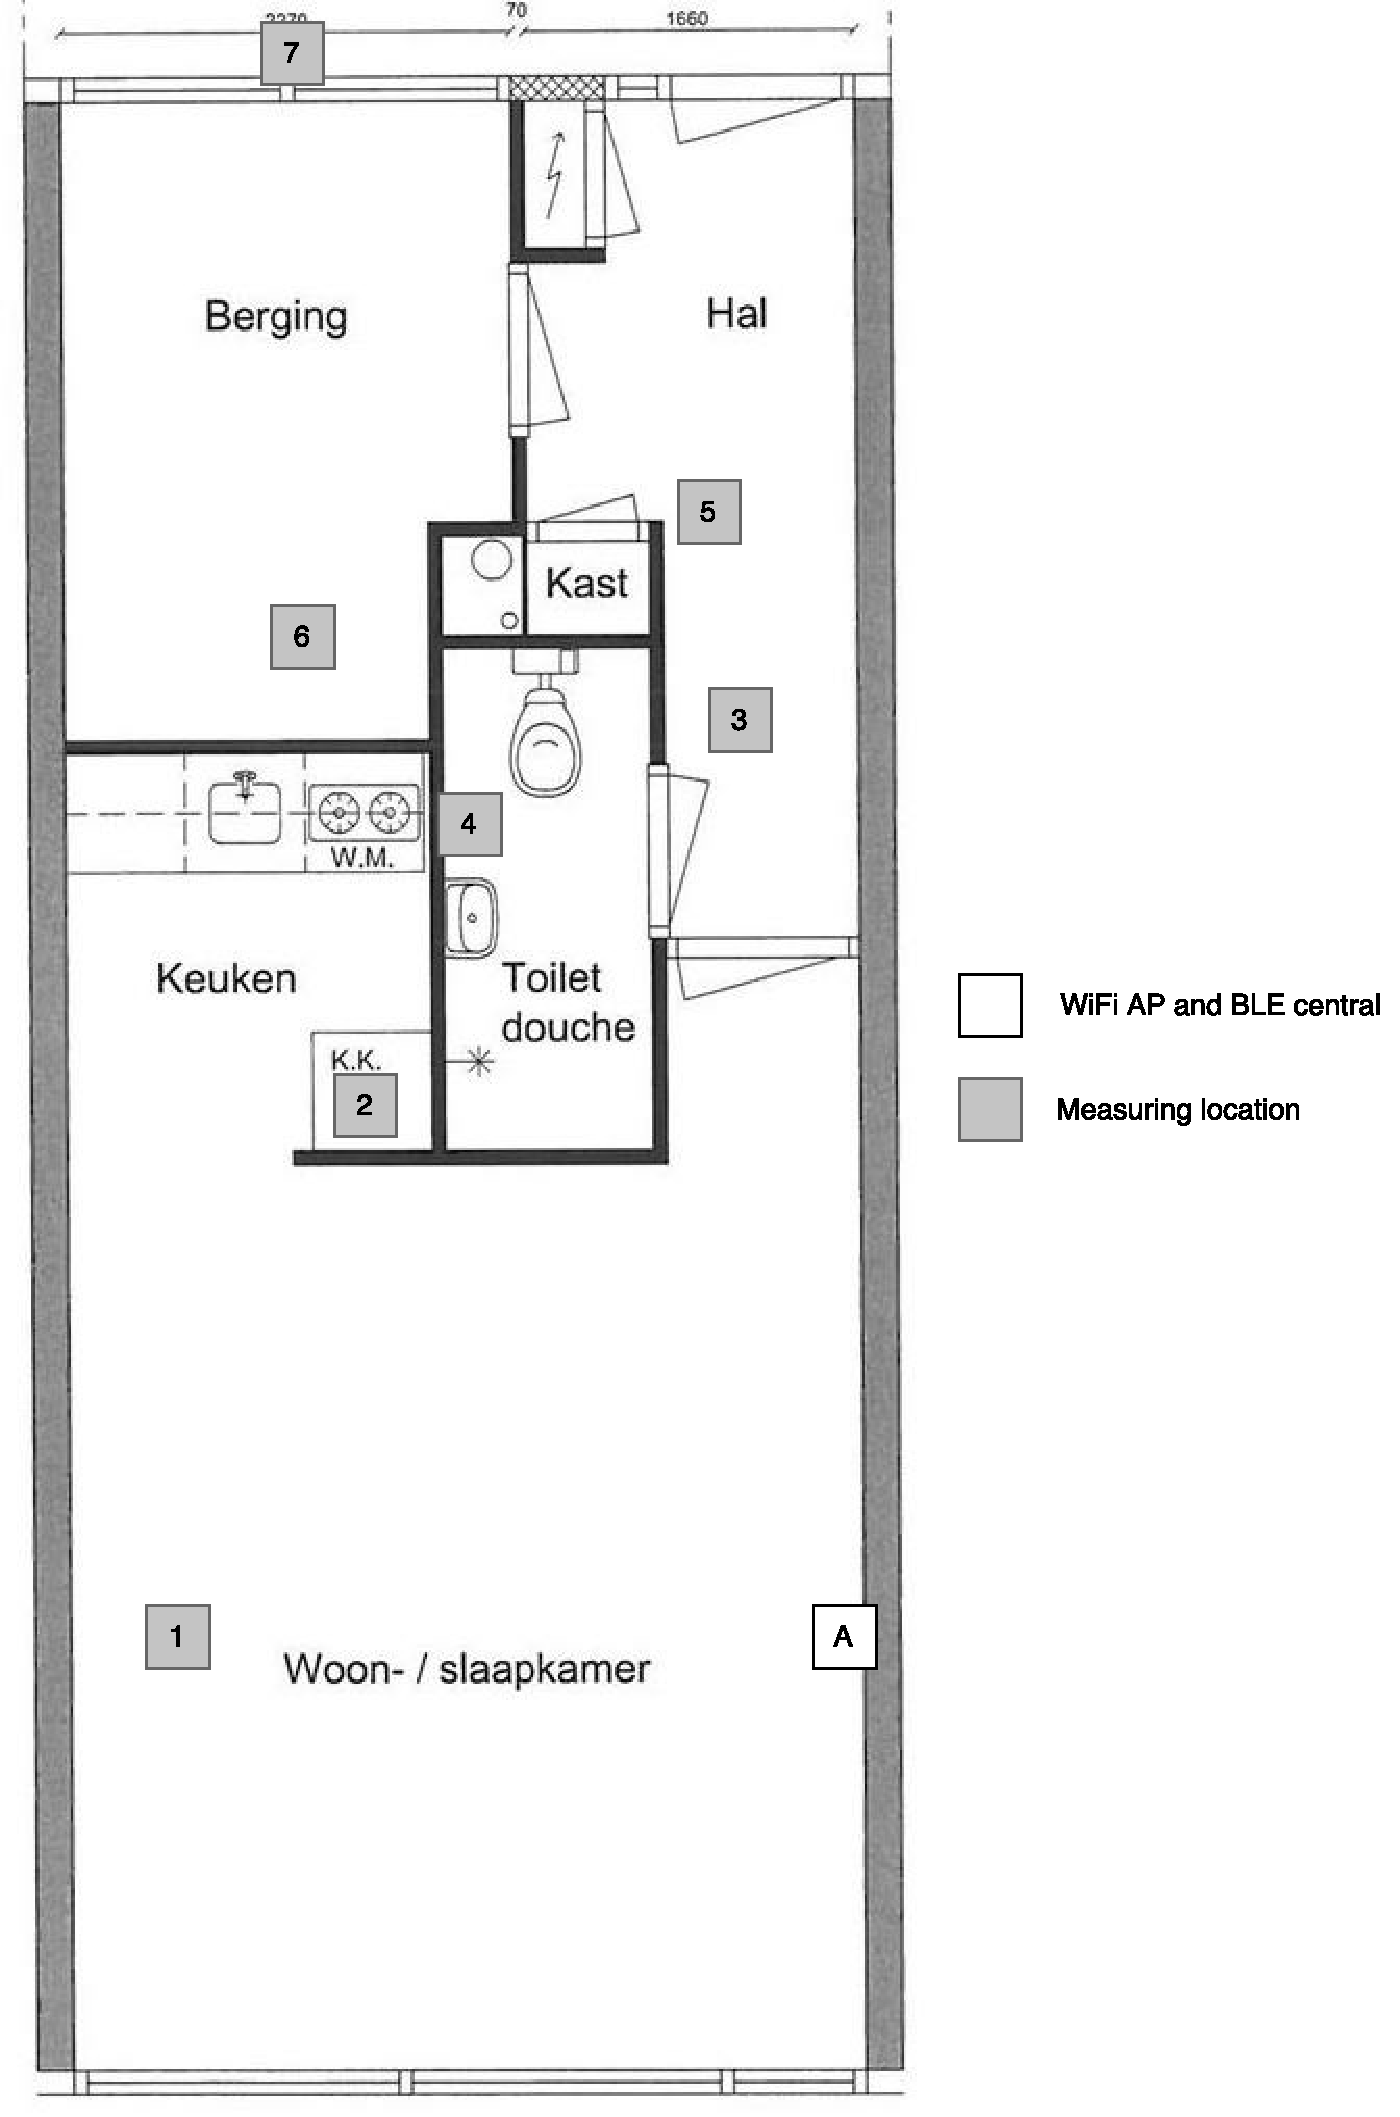
\includegraphics[width=0.37\textwidth]{experiment-map}
  \caption{A floor plan showing the location where the measurement takes place  and where the WiFi AP and BLE central are placed. Dark gray indicates Line of Sight communication (LoS), while light gray indicates non-LoS communication.}
  \label{fig:experiment-map}
\end{figure}

% where was it carried out?
The experiment was carried out in a Planetenlaan flat, Groningen, which has a living/bedroom, a kitchen, a toilet and shower room, and a storage room, as shown in Figure~\ref{fig:experiment-map}. The WiFi Access Point and the thin client is located in the right of the apartment next to the wall. There are seven positions of measurement in this case, in which even number indicates non-LoS, e.g., 2, 4, and 6, while odd number indicates LoS, e.g., 1, 3, and 5. The last position, 7, is added to measure the effect when the mobile phone is located outside the apartment. During the experiment, energy consumption is recorded when the mobile phone is positioned to each of the locations. Each experiment is measured in 3 minutes time interval.

[although the communications are different: BLE->iPhone to thin client; WiFi->iPhone to Access Point, both of the end points are located closely together]
[also add image about this]

% at mobile phone, what was done
At the time of experiment, flight mode was turned on to hinder Mobile data connection that may possibly affect energy consumption.  Background application may affect energy measuring result. Background App refresh in iOS is also disabled to prevent significant impact of background processes. When measuring WiFi communication, the Internet on the WiFi Access Point is disabled to prevent any running background application from fetching data from Internet through WiFi connection. Furthermore, only one means of communication is turned on during experiment, i.e., when recording HTTP over WiFi communication, WiFi is switched on and Bluetooth is switched off and vice versa.

% subsubsection measurement_parameters (end)

\subsection{Tailored Application Development} % (fold)
\label{sub:tailored_application_development}
Unlike~\cite{Balasubramanian2009} that uses common tasks in mobile phone, such as Internet browsing and emailing, a tailored application that meets the requirements described in Section~\ref{ssub:measurement_parameters}. This tailored application allows controlled environment that may focuses the energy measurement into several criteria, specifically for smart building application, with Azkario's architecture.

The application is written in Swift, which is the new general-purpose programming language developed by Apple Inc. Xcode, with Storyboard, is used to develop the application, with Git as the source code repository. A dummy occupancy data is sent to the server each time, as this study imitates the real implementation of user occupancy but not necessarily involves the sensing part. Each communication history is also saved using NSCoding in iOS for the sake of logging. The code is publicly stored in Github.com and is accessible at \url{https://github.com/gtrdp/cs-rug-internship}.

% screenshot of the app
\begin{figure}
    \centering
    \begin{subfigure}[b]{0.22\textwidth}
        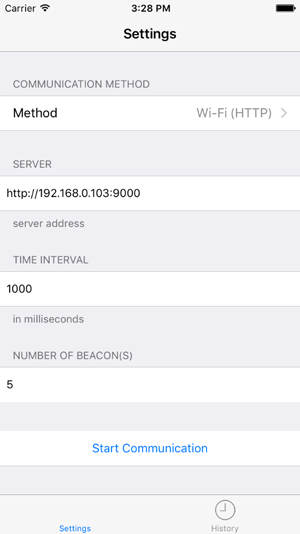
\includegraphics[width=\textwidth]{setting-screen}
        \caption{Setting screen.}
        \label{fig:setting-screen}
    \end{subfigure}
    ~ %add desired spacing between images, e. g. ~, \quad, \qquad, \hfill etc. 
      %(or a blank line to force the subfigure onto a new line)
    \begin{subfigure}[b]{0.22\textwidth}
        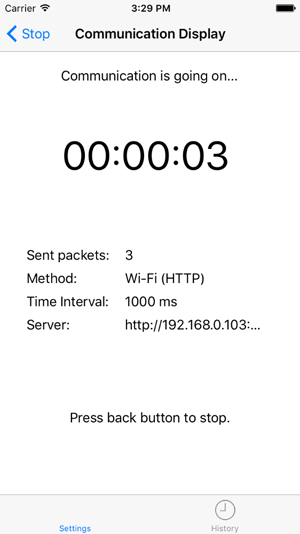
\includegraphics[width=\textwidth]{running-screen}
        \caption{Running screen.}
        \label{fig:running-screen}
    \end{subfigure}
    \caption{Screenshots example of the application showing a view for setting up the experiment (a) and a view showing the experiment progress (b).}\label{fig:screenshot-example}
\end{figure}

Figure~\ref{fig:screenshot-example} denotes two example of the application screenshots of the tailored application. As seen in Figure~\ref{fig:setting-screen}, the user could setting what communication method, the destination server, time interval (if needed), and number of beacon. When the measurement experiment is running, a progress screen is shown to the user that indicates the number of sent packets and current experiment runtime, as denoted in Figure~\ref{fig:running-screen}.

% Wifi
\subsubsection{WiFi Communication Scheme} % (fold)
\label{ssub:wifi_communication_scheme}
One of the communication method in the application is the WiFi communication. In this study, Alamofire library\footnote{\url{https://github.com/Alamofire/Alamofire}} is used to handle the HTTP communication as it encapsulates HTTP communication for easier and elegant use. A JSON object is sent via HTTP POST method in each time interval, i.e., 1000 ms, that contains occupancy data, as shown in Listing~\ref{lst-dummy-json}. The dummy data is derived from the real implementation of Azkario's architecture.

% give an example of dummy data in JSON
\begin{lstlisting}[caption=Example of dummy occupancy data in JSON., label=lst-dummy-json]
{
  "nearby_data":
    [
      {"data":{"proximity_zone":"NEAR",
               "proximity_distance":1.8456140098254021,
               "rssi":-81},
        "minor":1,
        "major":2222
      },
      {"data":{"proximity_zone":"FAR",
               "proximity_distance":3.171936276300526,
               "rssi":-87},
       "minor":2,
       "major":9999
      }
    ],
  "userId":"pratama"
}
\end{lstlisting}

Listing~\ref{lst-dummy-json} shows a JSON object that consists of two nearby beacons, denoted in JSON array, that is sensed by user with ID \texttt{pratama}. Each nearby data is composed of proximity data, which indicates the distance in meter and the signal strength, and beacon data, which is denoted by the major and minor number of beacon~\cite{AppleInc.2014}. If more beacons are set in the setting view, see Figure~\ref{fig:setting-screen}, \texttt{nearby\_data} object will have more element in its JSON array.

Moreover, a HTTP server is also built by using Play Scala framework in order to receive occupancy data. No logic is implemented in this HTTP server as this server only reads dispatched data and shows the reception timestamp.

% also explain about the server

% subsubsection wifi_communication_scheme (end)

% BLE
\subsubsection{BLE Communication Scheme} % (fold)
\label{ssub:ble_communication_scheme}
There are two main actors in BLE communication, the central and peripheral.  A peripheral is basically the device that owns the data, while a central is a device that uses the information presented by the peripheral to perform some desired jobs. Referring to the classic client-server architecture, a peripheral can be seen as a server that has the data and a central is the client who consumes the data. An illustration depicting central and peripheral device is shown in Figure~\ref{fig:central-peripheral}.

\begin{figure}[h!]
  \centering
    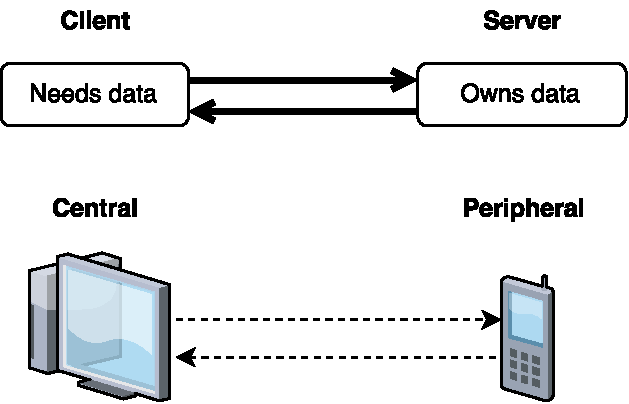
\includegraphics[width=0.3\textwidth]{central-peripheral}
  \caption{Central and peripheral device illustration.}
  \label{fig:central-peripheral}
\end{figure}

% brief introduction of BLE protocol
The way two BLE devices do data transmission is defined in Generic Attribute Profile (GATT)~\cite{BluetoothSpecialInterestGroup2014}. In this framework, GATT introduces concepts called Services and Characteristics. It utilizes a generic data protocol, namely Attribute Protocol (ATT), which is used to store Services, Characteristics and other related data.

According to~\cite{BluetoothSpecialInterestGroup2014}, there four main methods to make use of BLE communication from central to peripheral that are defined in Characteristics Value Declaration, namely read, write, indication, and notification. Read and write characteristics are self-explanatory, i.e., it is used to read or write data from or to the peripheral. Indication and notification are the methods for pushing the data to central, which is good to send continuous data, e.g., heart rate. The important difference is indication characteristic requires an application level acknowledgment for every transmission of data. On the other hand, notification characteristics does not manage the acknowledgments by the application.

% why notification is used and how to use it (subscription)
In this study, the iPhone, which provides occupancy data, serves as the peripheral, while the thin client acts as the central. Notification characteristic is used in this study because of its simplicity. Thus, the peripheral will advertise its characteristics with Unique User ID (UUID)~\cite{BluetoothSpecialInterestGroup2014} and the central will subscribe for this characteristics in order to get updated for notification.

% BLE packets
A dummy data is also sent in BLE communication, with the maximum user data in the packet is 20 bytes, as GATT protocol is used. This packet is relatively small to send occupancy data shown in Listings~\ref{lst-dummy-json}. That way, special format of data that can store all necessary data and fits with the constrains is created, as shown in Figure~\ref{fig:ble-packet-structure}. In this format, 20 bytes of data represents a single beacon. Thus, if more than one beacon has to be transmitted, the peripheral will transmit the packets multiple times, e.g., 10 times of transmission for 10 beacons.

\begin{figure}
  \centering
    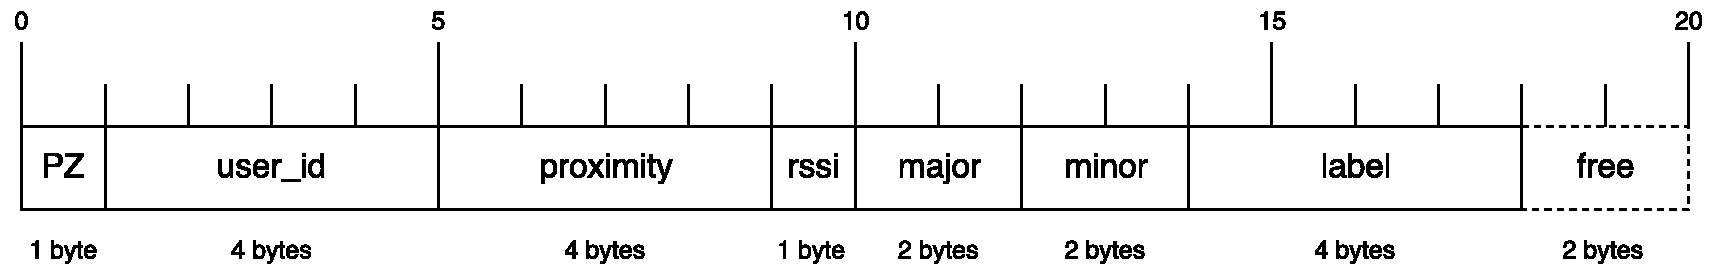
\includegraphics[width=0.51\textwidth]{ble-packet-structure}
  \caption{BLE packet structure consisting of occupancy data and user ID.}
  \label{fig:ble-packet-structure}
\end{figure}

The structure of the 20 bytes of data packet is depicted in Figure~\ref{fig:ble-packet-structure}. The packet starts with proximity zone, which is coded in \texttt{PZ}. This block may have two possibilities, either \texttt{NEAR} or \texttt{FAR}, which are coded in binary. The \verb|user_id| is coded in 32 bit unsigned integer and a mapping between those numbers with particular users are also created. The \verb|proximity|, encoded in floating point data type, discloses the distance between the user's mobile phone and the sensed beacon in meter. RSSI data is also incorporated in the structure, within \verb|rssi| block, while beacon information is stored in \verb|major| and \verb|minor| block~\cite{AppleInc.2014}. Referring to the JSON encapsulation of the occupancy data, shown in Figure~\ref{lst-dummy-json}, all beacons data are stored in single JSON file that marks out the same timestamp. The BLE implementation spreads those beacons data into single individual BLE packets, which would be separated and received in the BLE central in different timestamp. In order to overcome this problem, a random 32 bit unsigned integer \verb|label|, which marks those separated BLE packets into the same timestamp, is incorporated in the end of the packet. Two bytes of free space is left for further research.

% technical details

Speaking the technical implementation of the central application, initially Ian Harvey's bluepy library\footnote{\url{https://github.com/IanHarvey/bluepy}}, a Python interface to Bluetooth LE on Linux, was utilized. However, further development revealed that this library does not work to handle the notification characteristic in BLE. Subsequently, Sandeep Mistry's noble\footnote{\url{https://github.com/sandeepmistry/noble}} library, a node.js BLE central module, was later used. It turned out that it is capable to handle notification characteristic in BLE communication to subscribe the update of occupancy data. In the peripheral implementation, i.e., the iPhone, native Swift \verb|CBPeripheralManagerDelegate|, is used to handle BLE communication.

Furthermore, Bluetooth in noble is turned out to be a little bit unstable since it always loses the connection when it reached the 29th data packet. As a solution, the central application always tries to reconnect to the peripheral when it disconnected. Moreover, Bluetooth connection requires manual trigger to start scanning the nearby BLE devices. Thus, to accomplish the experiment efficiently, a VNC server is also set beside SSH server that is used to access the thin client remotely.
% subsubsection ble_communication_scheme (end)
% subsection tailored_application (end)
% section methodology (end)

\section{Results and Discussions} % (fold)
\label{sec:results_and_discussion}
The data measurement experiment was carried out for ten times for each parameters for both WiFi and BLE. The main results for WiFi and BLE measurements are presented in Figure~\ref{fig:wifi-result} and~\ref{fig:ble-result}.

\subsection{WiFi Communication Results} % (fold)
\label{sub:wifi_communication_results}
Figure~\ref{fig:wifi-result} presents the measurement results graph of WiFi communication between iPhone and the WiFi Access Point. The value is scaled from 0 to 20.As explained in Section~\ref{sub:tracing_}, the higher the value the more the iPhone consumes the energy or, in the other way, drains up the battery. The measurement is grouped based on the measurement location, numbered from 1 to 7, with each location consists of three combination of number of beacons, 5, 10, and 20, colored in green, blue, and yellow respectively. Measurement location number 1 to 6 are located inside the house, while number 7 is located outside the house. Furthermore, Line of Sight is incorporated in odd number of measurement location, while non-Line of Sight is in even number.

As the measurement location number increases, the distance between the WiFi Access Point and the iPhone increases as well. That way, such escalation of energy consumption is expected. However, such case is not found in the experiment. As seen in the measurement data number 1 to 6, the results seem to be fluctuating rather than increasing. An increase, however, is observed in the measurement number 7, in which the result exceeds 8 scale for 5 as the number of beacon. This case may be due to the location of the measurement which is outside the house. Moreover, there are also no differences of LoS and non-LoS communication. Small increasing is only observable in measurement number 3 and 4.

Other than the distance between the WiFi Access Point and the iPhone, the increasing of number of beacon is also assumed to intensify the energy consumption of the iPhone. However, the results asserts differently. As seen in all location of measurement, there are no clear trends that indicate energy increase. The only measurement that points an energy increase is only measurement number 3. Most measurements show that 10 number of beacon consumes least energy, as seen in measurement number 1, 2, 4, and 6. Surprisingly, the measurement number 7 shows a decline of energy consumption as the number of beacon decreases.

Summarizing those findings, there are no significant differences or trends in the WiFi energy measurement result. This situation may be caused by the distance difference that is not sufficiently far. The difference between each location is only one meter in length. Probably, significant difference could be noticed if the distance difference is increased. Furthermore, measuring the energy consumption using signal strength rather than distance can be an option.

% Wifi result
\begin{figure}
  \centering
    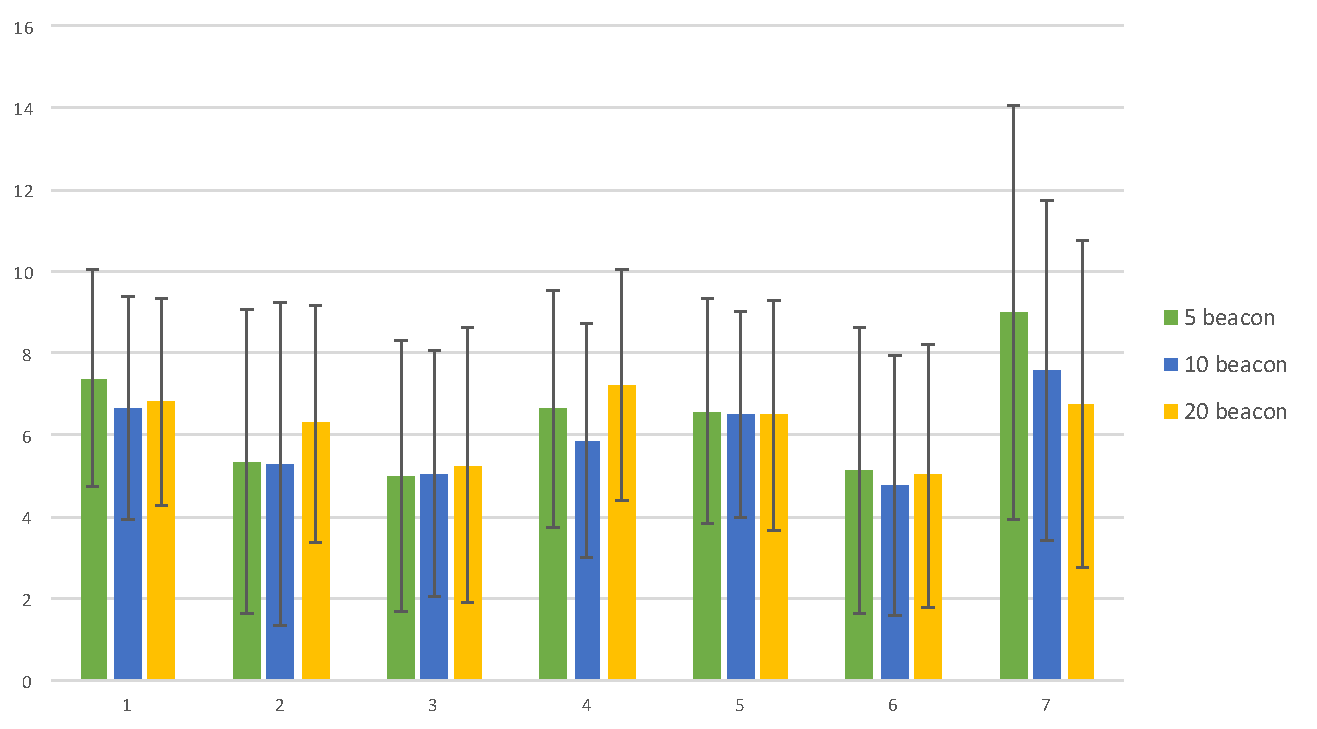
\includegraphics[width=.5\textwidth]{wifi}
  \caption{HTTP over WiFi measurement result.}
  \label{fig:wifi-result}
\end{figure}
% subsection wifi_communication_results (end)

\subsection{BLE Communication Results} % (fold)
\label{sub:ble_communication_results}
The BLE communication results, shown in Figure~\ref{fig:ble-result}, are also presented in the same way with the WiFi communication, i.e., it is grouped to 7 groups based on location, in which each location consists of three combination of number of beacon.

% Bluetooth result
\begin{figure}
  \centering
    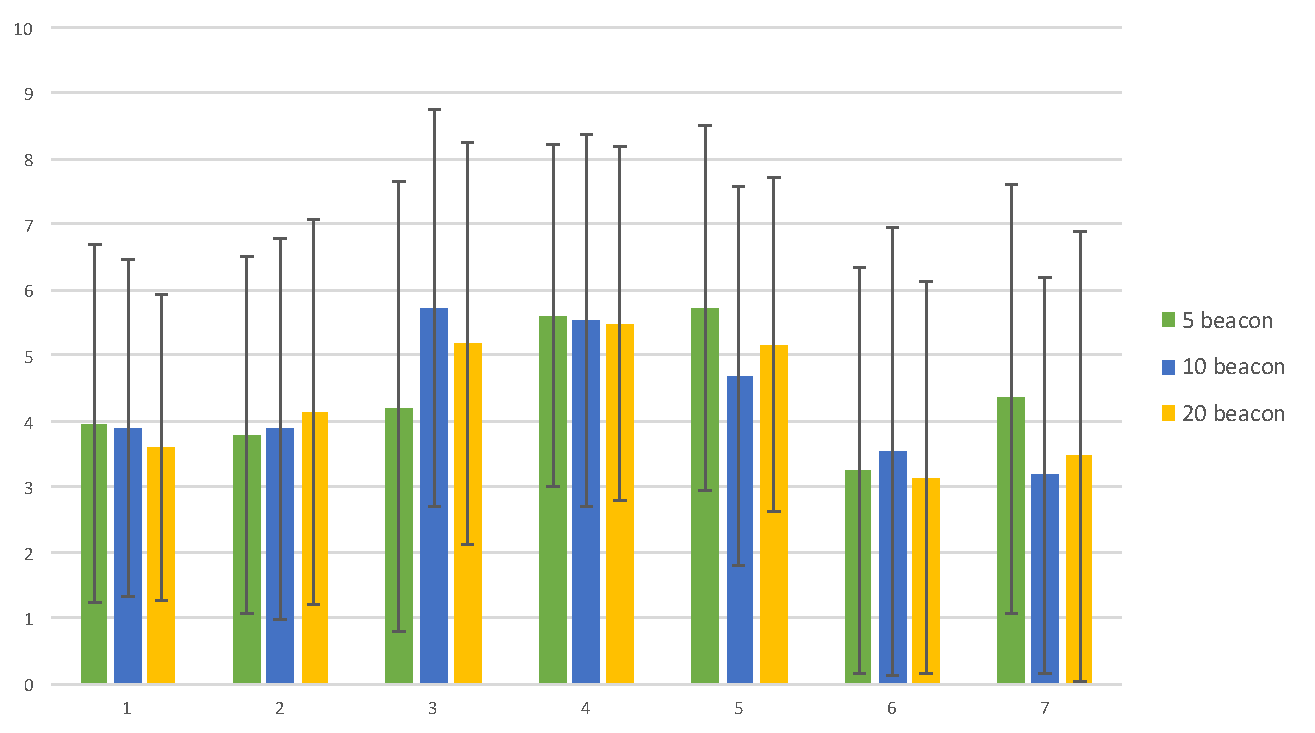
\includegraphics[width=.5\textwidth]{ble}
  \caption{BLE communication measurement result.}
  \label{fig:ble-result}
\end{figure}

The results of BLE energy consumption measurements also reveals slightly similar result with the WiFi energy measurements results. The results are also fluctuated and there are no such trends that marks out increasing energy consumption as the distance between iPhone and thin client increases. Looking at the LoS (odd number) and non-LoS communication, no significant differences are observable. Surprisingly, non-LoS communication in number 6 is much lower than the LoS counterpart, number 5. Unlike the WiFi counterpart, the last results of measurement, marked by number 7, does not significantly differ with the other measurement location.

No compelling trends or differences are observed, in terms of energy consumption for each number of beacon. Such relatively small increasing is only noticeable in measurement number 3, while small decreasing is observable in measurement number 1 and 4. The other measurements reveals fluctuating values. However, those disparities are not somewhat significant, i.e., not more than scale 2. These findings are somewhat similar with those found in WiFi measurement result.

In conclusion, no significant differences or trends in the BLE energy consumption measurement are found. Although a small gain from location 2 to location 3 is observed it is not sufficiently substantial. The same cause as the WiFi measurement might be the reason of these findings, which is insignificant measurement difference between one location to another, as these measurement are also based on the same measurement locations. Measuring using signal strength rather than communication distance would be an option to make the measurement yields expected results. However, this would lead to unbalanced comparison since WiFi signal strength is normally measured using dBm, while BLE is using RSSI.

% The highest value is not more than 6, which much lower than the highest value of 
% subsection ble_communication_results (end)


\subsection{Additional Results} % (fold)
\label{sub:additional_results}
In order to reveal more insights from the energy consumption comparison, the number of beacons are increased significantly for both of the communication methods. That way, the effect of packet size can be determined and a significant increase is expected to be present. Early testing revealed that it took roughly 4ms to send each BLE packet, i.e., sending 200 BLE packets would take around 800ms, which is lower than the sending interval (1000ms). Thus, current measurement uses 100 and 200 as the number of beacons because that is the limit to perform the communication without losing some packets.  Location 7 is selected to perform this measurement with the same parameters for the other configuration. The result is shown in Figure~\ref{fig:high-throughput}.

% WiFi and BT for high troughput
\begin{figure}
    \centering
    \begin{subfigure}[b]{0.13\textwidth}
        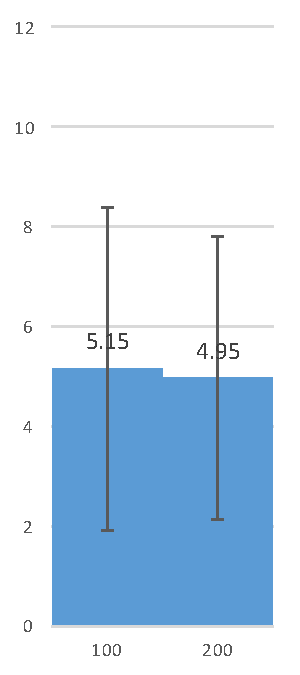
\includegraphics[width=\textwidth]{ble-high-tp}
        \caption{BLE energy consumption.}
        \label{fig:ble-high-tp}
    \end{subfigure}
    ~\quad %add desired spacing between images, e. g. ~, \quad, \qquad, \hfill etc. 
      %(or a blank line to force the subfigure onto a new line)
    \begin{subfigure}[b]{0.13\textwidth}
        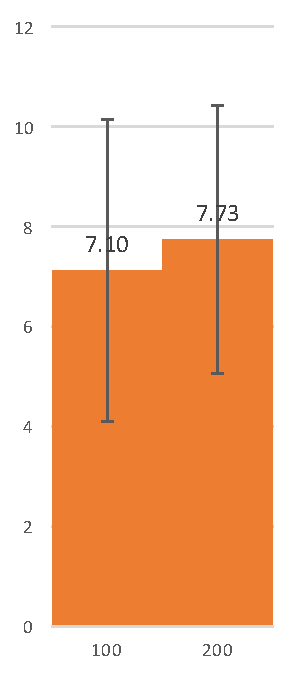
\includegraphics[width=\textwidth]{wifi-high-tp}
        \caption{WiFi energy consumption.}
        \label{fig:wifi-high-tp}
    \end{subfigure}
    \caption{Measurement result with 100 and 200 of beacons data for both BLE (1) and WiFi (2), measured in location 7.}
    \label{fig:high-throughput}
\end{figure}

As can be concluded from Figure~\ref{fig:high-throughput}, BLE communication consumes less energy than WiFi communication with roughly around 2 scale difference. However, there is no clear effect on the increase of the number of beacon in the results. The energy consumption slightly decreases by 0.2 in BLE communication, while WiFi communication energy consumption increases by 0.63. The change is relatively small, however. Thus, a conclusion can be drawn saying that there is no significant effect of the increase of number of beacon. Probably, the increase is quite small in size, i.e., bytes, so this small difference is actually consuming the roughly similar amount of energy, which leads to these results.

% final result, with baseline
Previously, detailed results of energy measurements with arranged parameters for both WiFi and BLE have been presented. However, no direct comparison for both main communication is shown. In order to compare the energy consumption directly, a baseline energy consumption is introduced. It is a measurement in which no unnecessary processes or communications present in the iPhone. That way, all of communication means are switched off, e.g., 4G, WiFi, and Bluetooth, and all of installed applications are halted. Some background processes, however, are still able to interfere the experiment by consuming some energy unexpectedly, although it would be in a small effect. As previous measurements, this experiment is also carried out within 3 minutes of time frame and repeated for 10 times. The result is depicted in Figure~\ref{fig:baseline-ble-wifi}.

\begin{figure}
  \centering
    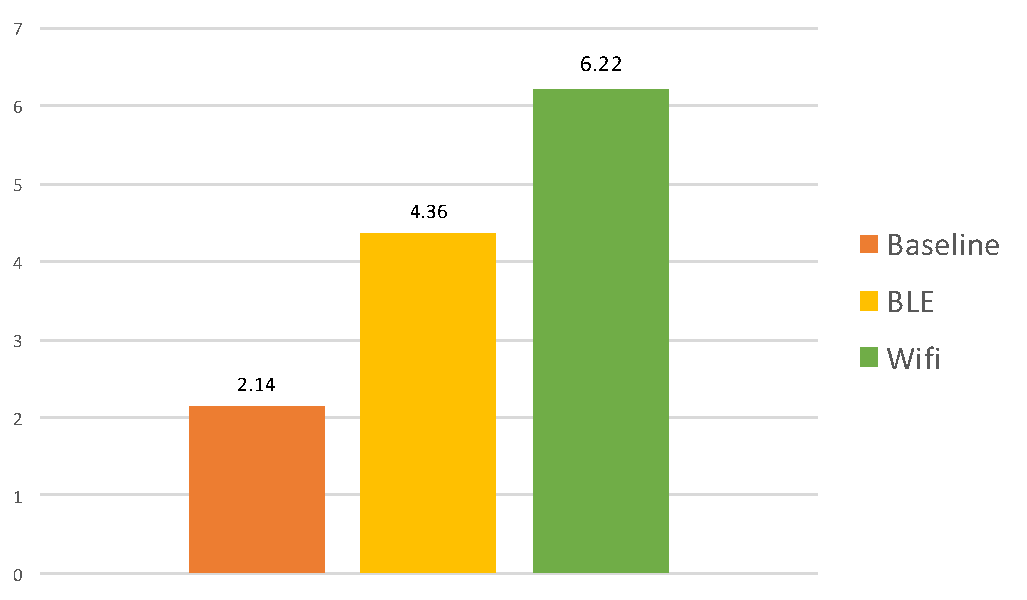
\includegraphics[width=.5\textwidth]{baseline-ble-wifi}
  \caption{The average of energy consumption for both BLE and WiFi along with baseline energy consumption as a comparison.}
  \label{fig:baseline-ble-wifi}
\end{figure}

Based on the measurements, the baseline energy consumption is nearly 2.15 out of 20 in average. According to the scale conversion in Section~\ref{sub:tracing_}, this value means that the iPhone will have 18 hours and 51 minutes of battery life when set in the baseline configuration. As the iPhone is totally passive, i.e., no applications are running and all means of communication are switched off, this durability is somewhat low. However, the standard deviation is also fairly high, which is counted 2.6.

Figure~\ref{fig:baseline-ble-wifi} also presents the average value of BLE and WiFi energy consumption, which are 4.36 and 6.22 respectively. This value indicates that the iPhone will have 16 hours and 38 minutes of battery life in BLE communication and 14 hours and 46 minutes in WiFi. Based on this measurements, BLE is proven to be 29.97\% more energy efficient than WiFi. This result is may limited only to smart building application because the metrics and the parameters used in this study are devised for smart building application.

% subsection additional_results (end)

% section results_and_discussion (end)

\section{Conclusion} % (fold)
\label{sec:conclusion}
% is it ok to add more findings or insights in conclusion, which are not presented in the previous chapters?
Bluetooth Low Energy (BLE) and WiFi are the most popular means of communication in current modern smart phones. As most of the recent smart phones, ranging from the entry level to the top class phone, own that, such opportunities to make use of them for solving problems in smart buildings are present, for instance, the application of BLE and WiFi to solve occupancy problems. This study has presented the comparison of energy consumption in BLE and WiFi communication, specifically for the case of occupancy detection in smart buildings. This study only focuses on the energy consumption of the transmission of occupancy data from the user's mobile phone to the communication end points, e.g., WiFi Access Point or BLE central.

% how to achieve that
In order to investigate the energy consumption in transmitting occupancy data, some parameters are designed, such as the number of beacon sensed and the distance between those communication end points with Line of Sight and non-Line of Sight communication. A tailored application is also developed to support the measurement using those parameters.As this study only focuses on transmitting the data, no sensing activity is performed and dummy occupancy data is sent.

% what is the result
The result alleges that BLE is actually 29.97\% more energy efficient than WiFi to transmit occupancy data from user's smart phone to the communication endpoints. According to the measurement statistics, the smart phone has 16 hours and 38 minutes of battery life when running on BLE communication scheme and 14 hours and 46 minutes in WiFi communication. However, no significant effect are observed on parameter change.

% some discussion for drawbacks or comments or future works
Instability was observed during BLE experiment that might be caused by the BLE central library's bug or some code smells in the central applications.

In the experiment, brightness was proven to be one of significant source of energy loss as it consumes much energy to light up the screen.

Limitation: only tested for iPhone 6 running iOS 9.3.2.
Brightness is one factor.

Wifi may still be a consideration because usually mobilephone are also using wifi extensively.
Explain the pros and cons regarding the implementation of Bluetooth as replacement of WiFi. A protocol must be devised to prevent bottleneck in accessing Bluetooth.

% section conclusion (end)


%% if specified like this the section will be committed in review mode
\acknowledgments{
The authors wish to thank A, B, C. This work was supported in part by
a grant from XYZ.}

\bibliographystyle{abbrv-doi-hyperref-narrow}
\bibliography{cs-rug-internship.bib}
\end{document}

